\chapter{Reprezentace sítí MHD}
Data o~různých cestních sítích obvykle ukládáme ve formě grafu, ve kterém pak
vyhledáváme jednotlivé trasy pomocí prohledávání grafu, na které existuje mnoho
známých algoritmů. Pokud ale potřebujeme udržovat kromě dat o~cestní síti data
o~jízdních řádech, stává se situace mnohem složitější, protože zatímco po cestách
můžeme jít kdykoli, cestovat hromadnou dopravou můžeme pouze tehdy, když zrovna
jede nějaký spoj. Pro reprezentaci sítí hromadné dopravy se vyvinuly různé
způsoby, dále představíme nejobvyklejší z~nich.

\section{Time expanded modely}
Time-expanded modely\cite{time-expanded} jsou konstruovány tak, aby ceny hran
byly konstantní a šlo na takovýto graf použít běžné vyhledávání v~grafu.
V~těchto modelech jsou jako vrcholy dvojice (zastávka, čas odjezdu) a (zastávka,
čas příjezdu) pro každý čas odjezdu a příjezdu z~každé zastávky. Hrany pak
jsou jednak \uv{spojové} spojující vždy dvojici odjezd-příjezd mezi dvěma
zastávkami pomocí nějakého spoje, jednak \uv{čekací}, které spojují jednotlivé
časy v~rámci jedné zastávky tak, jak jde čas. Spojení pak hledáme tak, že na
množině vrcholů patřících k~výchozí zastávce najdeme vrchol s~nejbližším vyšším
časem, než je náš odjezdový. Běžným průchodem do šířky podle času přes spojové a
čekací hrany pak najdeme cestu do cílové zastávky. Nevýhodou této reprezentace
je velikost grafu.

Tento základní model nerespektuje časy potřebné pro přestup, což může být
zvlášť problematické u~rozsáhlých stanic či zastávek s~mnoha zastávkovými
stojany. Tento problém se dá vyřešit rozdělením linie událostí u~jedné zastávky
na více. Vrcholy patřící k~jedné zastávce rozdělíme na zastávkové, příjezdové a
odjezdové. Odjezdové vrcholy odpovídají odjezdům spojů ze zastávky a příjezdové
vrcholy příjezdům do zastávky. Zastávkové vrcholy odpovídají každý jednomu
odjezdovému vrcholu. Zastávkové vrcholy jsou spojeny hranami do posloupnosti
stejně jako v~původním grafu. Z~příjezdového vrcholu vedou hrany do nejbližšího
zastávkového vrcholu, do kterého se stihne pěší přesun a do všech dřívějších
odjezdových vrcholů, do kterých se stihne pěší přesun, viz obr.
\ref{fig:time-expanded}. Ze zastávkového vrcholu
vede navíc hrana do odpovídajícího odjezdového vrcholu. Všechny přestupní hrany
mohou být ohodnocené potřebným časem na přestup mezi linkami. 
\begin{figure}[h]
  \centering
    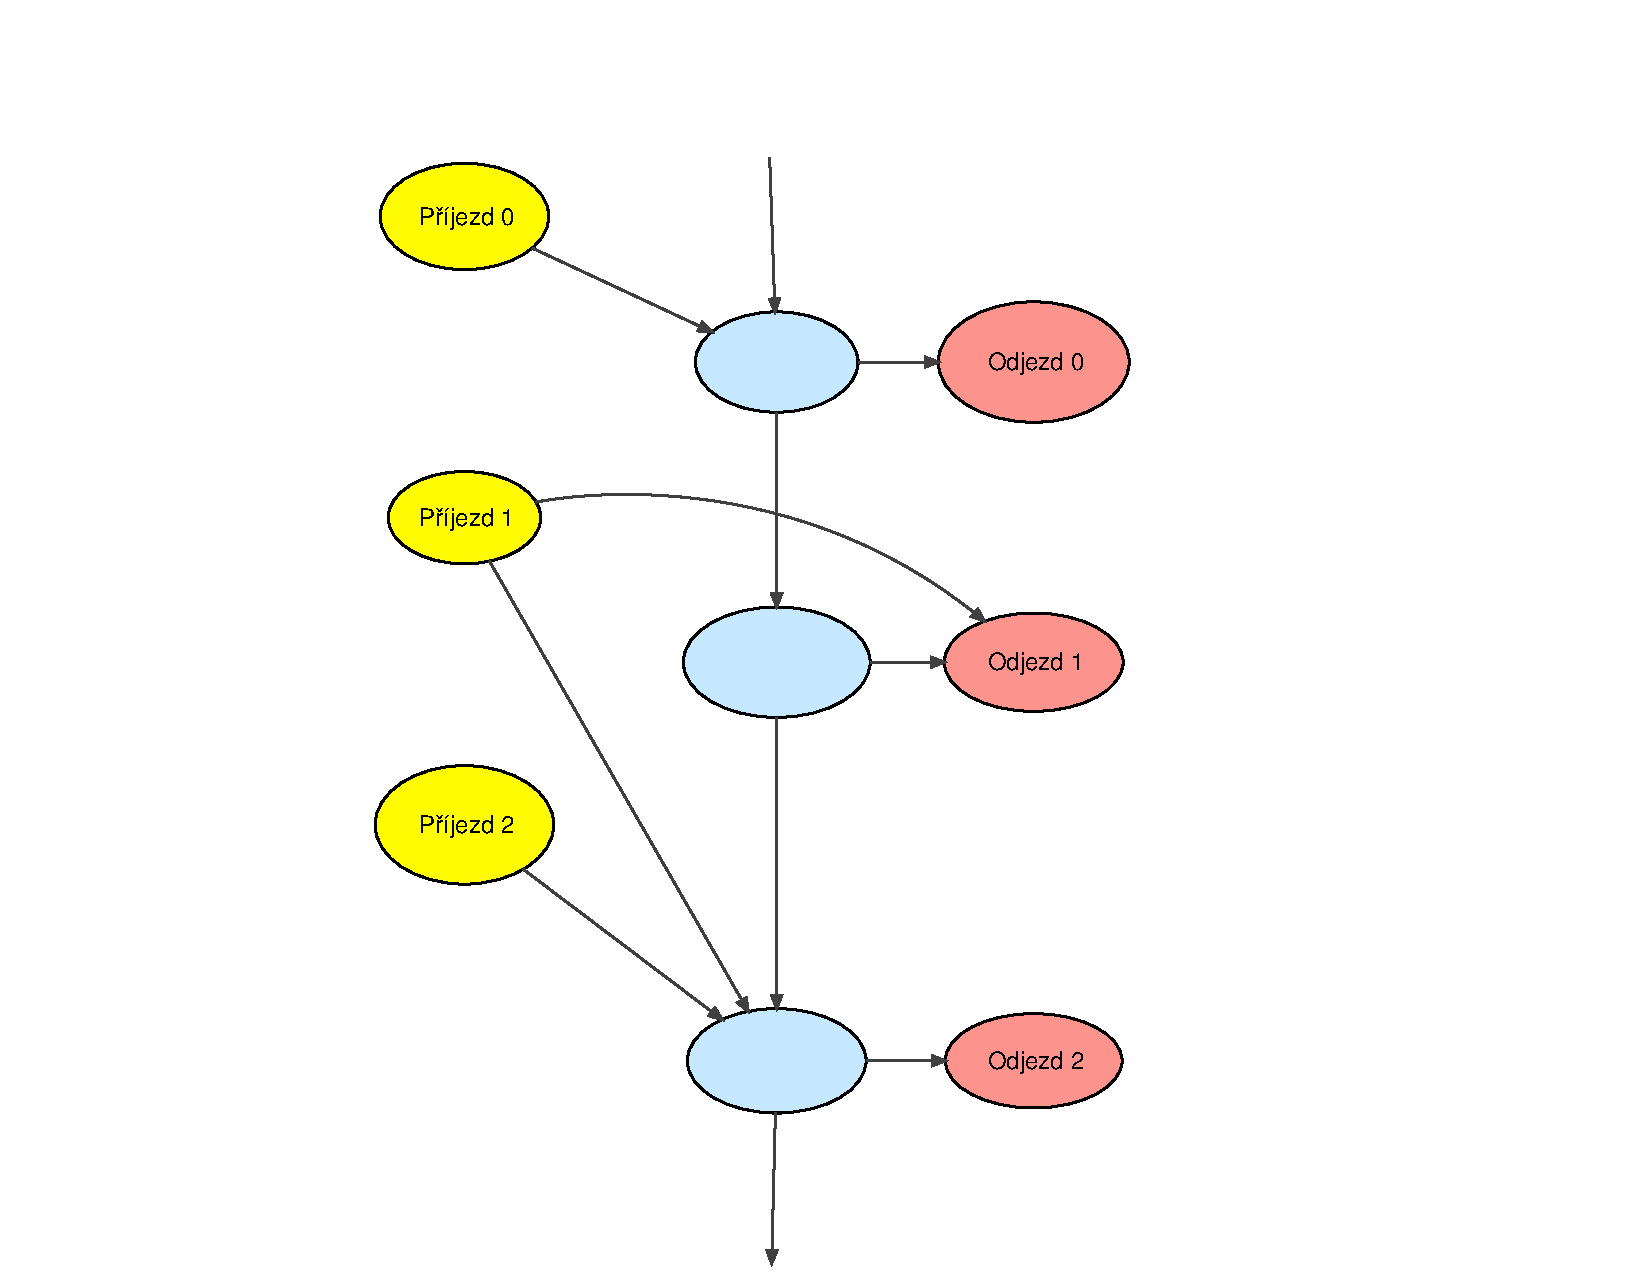
\includegraphics[scale=1.5]{../img/time-expanded.pdf}
  \caption{Příjezdové (žlutě), odjezdové (červeně) a zastávkové (modře) vrcholy.
  Všimněte si, že z příjezdu 1 lze stihnout odjezd 1, ale jen proto, že jsou
  blízko sebe, obecný spoj odjíždějící ze zastávky v čase odjezd 1 bychom
  nestihli.}
  \label{fig:time-expanded}
\end{figure}

\section{Time-dependent modely}
Time-dependent modely\cite{time-dependent} se snaží odstranit problém
s~velikostí grafu hromadné dopravy. Místo toho, abychom měli pro každý spoj
zvláštní hranu, sdružíme spoje do linek, kde všechny spoje jedné linky mají
stejnou posloupnost zastávek. Vrcholy tentokrát budou jen jeden pro každou
zastávku. Hrany mezi zastávkami budou jedna pro každou linku, která danou
dvojici zastávek spojuje. V~takovémto grafu již nemůžeme vyhledávat pomocí
běžného průchodu grafem, potřebujeme mít upravenou funkci, která vyhledá
v~jednotlivých časech odjezdu pro každou linku nejbližší od okamžiku příjezdu do
zastávky. Tento přístup nevytváří grafy s~velkým počtem vrcholů a hran, navíc je
tato reprezentace snáze připojitelná do vyhledávacího grafu pro obyčejnou cestní
síť.

Existuje také varianta, která má jeden staniční vrchol a
pro každou linku projíždějící danou stanicí linkový vrchol. Tyto vrcholy jsou
pak propojeny přestupovými hranami a umožňují realističtější modelování
rozsáhlejších stanic a přestupů v~rámci nich. Ani tento model však nevyužívá
všech vlastností spojů MHD, jako je například to, že spoj má danou trasu a že
když na něj někde nastoupíme, tak snadno můžeme do dalšího vyhledávání přidat všechny
průjezdní stanice.  

\section{Contraction hierarchy}
Contraction hierarchy\cite{CH} je způsob předzpracování dat tak, aby následné
vyhledávání nemuselo procházet celý graf. U~cestní sítě tomu odpovídá obvyklý
postup při cestování -- nejprve cestujeme po místních silnicích, abychom se
dostali na silnice první třídy a dálnice, po těch pak dojedeme blízko cíle, kde
opět přecházíme na místní silnice, abychom dosáhli cíle. U~cestní sítě se
příprava dat provádí obdobně -- jsou nalezeny významné body, přes které
přecházíme na silnice vyšších tříd a cesty na dlouhé vzdálenosti jsou pak
rozděleny na hledání cesty do významných bodů a hledání cesty mezi nimi. Tato
hierarchie může mít i několik stupňů a cesty mezi výzmanými body jsou často
předpočítány.

Obdobně se dá vytvořit podobná hierarchie i u~hledání spojení MHD, kdy si
udržuji zkratky mezi uzlovými zastávkami a nemusíme pak prohledávat jednotlivé
mezilehlé zastávky, kde stejně nemůžeme na nic přestoupit. Problém této
reprezentace pro nás je s~přidáváním pěších tras, protože je potřeba mít všechny dopředu
spočítané. Předvýpočet je stejně tak problematický i u~cestní sítě, protože
předpokládá pevné nastavení cestovních rychlostí a preferencí cest, na základě
kterých jsou nalezeny ulzové body a vypočítány zkratky. Náš cíl je umožnit
uživateli tyto parametry si zvolit při hledání dle svých potřeb, proto pro nás
není tento model vhodný. 

\section{RAPTOR}
RAPTOR (Round-Based Public Transport Routing)\cite{RAPTOR} je oproti
time-dependent modelům založen na zcela odlišných myšlenkách a při svém běhu
nevyužívá algoritmy pro procházení grafu. RAPTOR se snaží využít co nejvíce vlastností,
kterými se odlišuje síť veřejné dopravy od obyčejné cestní sítě. Také umožňuje
snadno optimalizovat na počet přestupů.

Algoritmus pracuje po kolech. Každé kolo znamená nástup do dalšího dopravního
prostředku, celkově je tedy počet kol o~1 větší než maximální počet přestupů.
Algoritmus pracuje s~linkami. Každá linka má několik spojů, což jsou konkrétní
vozidla, která všechna projíždí stejnou posloupnost zastávek ve stejném směru. Každý spoj má
uloženy časy odjezdu z~jednotlivých zastávek, předpokládáme, že se dva spoje
jedné linky na trase nepředjíždí. Pro každou zastávku si pro každé kolo
pamatujeme, zda a kdy je dosažitelná pomocí kterého kola. Nedosažitelnost
zastávky reprezentujeme pomocí nastavení času příjezdu v~daném kole na $\infty$.

Na začátku jsou všechny zastávky ve všech kolech nedosažitelné. Nastavíme
výchozí zastávce čas dosažení v~prvním kole na zadaný čas odjezdu a spustíme
algoritmus. Ten postupně prochází linky po jejich zastávkách a pokud narazí na
dosažitelnou zastávku, tak najde nejbližší spoj linky, který z~dané zastávky
odjíždí po čase dosažitelnosti a tímto spojem se \uv{vydá} a průběžně upravuje
časy dosažitelnosti na dalších zastávkách. Pokud po cestě nalezne další
dosažitelnou zastávku, jako spoj z~této zastávky vybere z~původního spoje a
spoje navazujícího na původní čas dosažitelnosti ten, který odjíždí dříve. Takto
pokračuje až do konce linky. Po průchodu všech linek se všechny časy
dosažitelnosti zkopírují do dalšího kola a algoritmus se znovu spustí. Po
stanoveném počtu kol algoritmus skončí a u~jednotlivých zastávek je pro každé
kolo (odpovídající počtu přestupů $- 1$) uloženo, zda je s~daným počtem přestupů
dosažitelná a v~jakém čase. K~jednotlivým časům u~zastávek je vhodné si uložit
linku, která způsobila úpravu na daný čas, abychom byli schopni zrekonstruovat
spojení využité k~dosažení dané zastávky. 

Tento algoritmus je snadno implementovatelný a při vhodně zvolených datových
strukturách velmi rychlý a vhodně využívající keš. 

\subsection{Uložení dat}
\label{ch:reserse:raptor-data}
Pro rychlý výpočet a efektivní využití keše je potřeba mít vhodně uložená data.
Data stejného typu jsou vždy uložená v~poli za sebou. Pokud různé objekty mají
každý mít seznam stejného typu, jsou všechna data od všech objektů držena
v~jednom poli a každý objekt si drží počet svých prvků a odkaz na první z~nich.
Tímto má každý objekt vyhrazen svůj úsek a může s~ním efektivně pracovat. Tento
mechanismus nazveme \uv{polním mechanismem} a budeme na něj takto odkazovat ve
zbytku kapitoly.

Základem pro prohledávání je pole linek. Každá linka má odkaz na své zastávky a
na časy zastavení spojů v~zastávkách. Obojí je implementováno polním mechanismem
a rozdělení na zastávky a spoje zajišťuje snadnou možnost hledání spojů v~daný
čas. Časy zastavení spojů v~zastávkách jsou uspořádány v~poli za sebou podle
zastávek a pak podle času výjezdu spoje z~výchozí zastávky. Protože
předpokládáme, že se spoje nepředjíždí a všechny spoje jedné linky mají stejný
počet zastávek, na předchozí spoj snadno přejdeme skokem v~poli zastavení
o~počet zastávek linky vzad, následující spoj najdeme obdobným skokem vpřed. Také
je možné pro konkrétní zastávku a konkrétní čas použít jednoduše binární
vyhledávání pro nalezení nejbližšího spoje odjíždějícího po konkrétním čase. 

Pro vyhledávání z~konkrétní zastávky máme obdobně implementovány datové
struktury kolem zastávek. Zastávky jsou uloženy v~poli za sebou, každá si drží
seznam linek, které jí projíždějí, a seznam pěších přestupů z~dané zastávky. 
Obojí je reprezentováno polním mechanismem.   

